% !TeX root = AstCreator.tex
\definecolor{dkgreen}{rgb}{0,0.6,0}
\definecolor{gray}{rgb}{0.5,0.5,0.5}
\definecolor{mauve}{rgb}{0.58,0,0.82}
\lstnewenvironment{astlst}[1][]%
{\lstset{basicstyle=\footnotesize\ttfamily,language=Java, morekeywords={Packages,Tokens,Abstract,Syntax,Tree,Aspect,Declaration},frame=single,stringstyle=\color{mauve},commentstyle=\color{dkgreen}}#1}
{}



\section{Syntax}

The syntax is divided into a number of sections:

\begin{description}

\item[\textbf{\texttt{Packages}}] This section allowed the default packages to be defined for \texttt{base} that forms the basis for all nodes if nothing else is specified and \texttt{analysis} where all visitors will be generated under:

\begin{astlst}
Packages
base org.overture.ast.node;
analysis org.overture.ast.analysis;
\end{astlst}

\item[\textbf{\texttt{Tokens}}] This section defines tokens or external nodes that can be used as fields in the AST. \textit{The important part here is that they must be clonable}. The following types of tokens can be specified:
\begin{description}
\item [Token] A token is an instance of the class \texttt{Token}, it is automatically generated from a name plus the text it represents.

\item [Standard Java Types] Standard Java types (basic types) can be used in the class form. The use of those relies on them being parse by value when cloning is done. E.g. \texttt{Integer, Boolean, Long, Character, ...}

\item [External Java enum] This is like the standard Java type where the type given is a Java \texttt{enum}.

\item [External classes] Any external class can be used as a field in the AST but it must implement the interface \texttt{ExternalNode} that provides a handle to the AST for proper cloning for the node.

\item [External defined Node] This enables a node to be specified outside the AST creator but still included in the analysis. The class must extend \texttt{Node} and do a proper implementation of the analysis methods and kind methods returning the correct enumeration.

\end{description}

\begin{astlst}
Tokens
//Token 
bool = 'bool'; 
//Standard Java Type
java_Integer = 'java:java.lang.Integer'; 
//External Java enum
nameScope = 'java:enum:org.overturetool.vdmj.typechecker.NameScope';
//External Java type
location = 'java:org.overturetool.vdmj.lex.LexLocation'; 
//External defined node
LexToken = 'java:node:org.overturetool.vdmj.lex.LexToken'; 
\end{astlst}

\item[\texttt{Abstract Syntax Tree}] This section describes the tree. Names at the top level are considered roots and \# are considered sub roots. Sub roots must be  specified as a root and a child. 

\begin{astlst}
Abstract Syntax Tree
exp {-> package='org.overture.ast.expressions'}
    =   {binary} [left]:exp [op]:binop [right]:exp
    |   ...
    ;

binop {-> package='org.overture.ast.expressions'}
    = {and}
    |   {or}
    |   ...
    ;
\end{astlst}


%#Unary {-> package='org.overture.ast.expressions'}
%    =   {absolute} 
%    |   {head} 
%    |   {mapInverse} (mapType):type.#Map
%    ;

The above example will generate a tree like:
\begin{figure}[htb]
\begin{minipage}{0.5\linewidth}

\texttt{
\Tree[.exp [.binary left:exp op:binop right:exp ] ]}
\caption{AST Example.}

\end{minipage}
\begin{minipage}{0.5\linewidth}

\texttt{
\Tree[.PExp [.ABinaryExp left:PExp op:PBinop right:PExp ] ]}
\caption{AST Java Generated code Example.}

\end{minipage}
\end{figure}

\begin{description}
\item [The type of field]:
Fields can be specified in two different ways:
\begin{description}
\item[Tree]: Tree fields are fields that belong to a single node in tree and only that one. A tree node cannot be a child of any other node in the tree. Thus if an instance is assigned to a tree field the parent it may belong to is disconnected such that the child/parent relation ship is preserved.\\
Tree fields are syntactically specified as: \texttt{[feld]:type}, where \texttt{field} is the name and \texttt{type} is the type name.
\item[Graph]: Graph fields are reference fields thus the get parent will not deterministically return a single parent but just the first parent the instance was added as a reference field of. This type of node can e.g. be used to add type information to nodes where the type is a reference to a shared type. \\
Tree fields are syntactically specified as: \texttt{(feld):type}, where \texttt{field} is the name and \texttt{type} is the type name.
\end{description}

\item [Field types]:
Fields must define the type of the field as a name reference to a tree element like shown in listing~\ref{} above. The syntax is \texttt{:type} where the type can be any of the below shown references:
\begin{description}
\item[Simple types]: Simple types is just the type name like \texttt{:exp} or if a nested type is given \texttt{exp.\#unary.abs}
\item[Lists]: Lists are specified as simple types but appended with a star \texttt{:exp*}
\item[Double lists]: List simple types but with two stars \texttt{:exp**}
\end{description}

\item [Sub-classing]: A sub class can be made by specifying a root as an alternative of another root. The naming convention dictates that the sub class roots must begin with \#. E.g.:

\begin{figure}[htb]
\begin{minipage}{0.5\linewidth}

\texttt{
\Tree[.exp \#unary ]}
\\
and
\\

\texttt{
\Tree[.\#unary abs minus ]}
\caption{AST Example.}

\end{minipage}
\begin{minipage}{0.5\linewidth}

\texttt{
\Tree[.PExp [.SUnaryExp AAbsUnaryExp AMinusUnaryExp ] ]}
\caption{AST Java Generated code Example.}

\end{minipage}
\end{figure}

\end{description}

\item[\textbf{\texttt{Aspect Declaration}}] This is a feature that allows any fields to be added to base classes (root classes in the AST grammar, the nodes where a a package can be specified). One example could be to add a \texttt{location} field to all nodes of the \texttt{exp} type. The field will be the first declared field in any of the sub classes of \texttt{exp}. The syntax looks like this:

\begin{astlst}
Abstract Declaration
%exp = [location]:location
    ;
\end{astlst}
Where \% prefixes the root node name. The name can also be a composite name like \texttt{\%exp.\#unary}.

\end{description}

\subsection{Usage}
The ast generator can be invokes like: 

\begin{astlst}
java -cp astCreator.jar com.lausdahl.ast.creator.CmdMain ast.astV2 .
\end{astlst}

\subsection{Extensions}

%\subsection{Extendibility and Isolation of Additions}\label{sec:astExtendIsolation}

%\begin{itemize}
%\item The general idea about creating a new grammar file and adding only the new stuff, new fields and nodes.
%\item First proposal isolate changes and make a new AST. Not a good idea. No reuse at all
%\item Solution creating a new subclassed AST with the additions.
%\item Create
%\end{itemize}

In this subsection we describe a new way to specify and generate a tree that extends a base tree and preserves backwards compatibility with its base tree. Extensions are only visible to components that depend on the extended tree otherwise only the base tree structure will be accessible. In figure~\ref{fig:ast_extensions} examples of extensions required by Overture is shown. Each box defines a plug-in feature that needs its own extensions like a type field to store the derived type information from a type checker and a proof obligation generator needs a place to attach proof obligations. The figure also illustrates that an extended tree may be further extended; In this case the derived type information is needed by the interpreter. 

\begin{figure}[tbh]
\centering
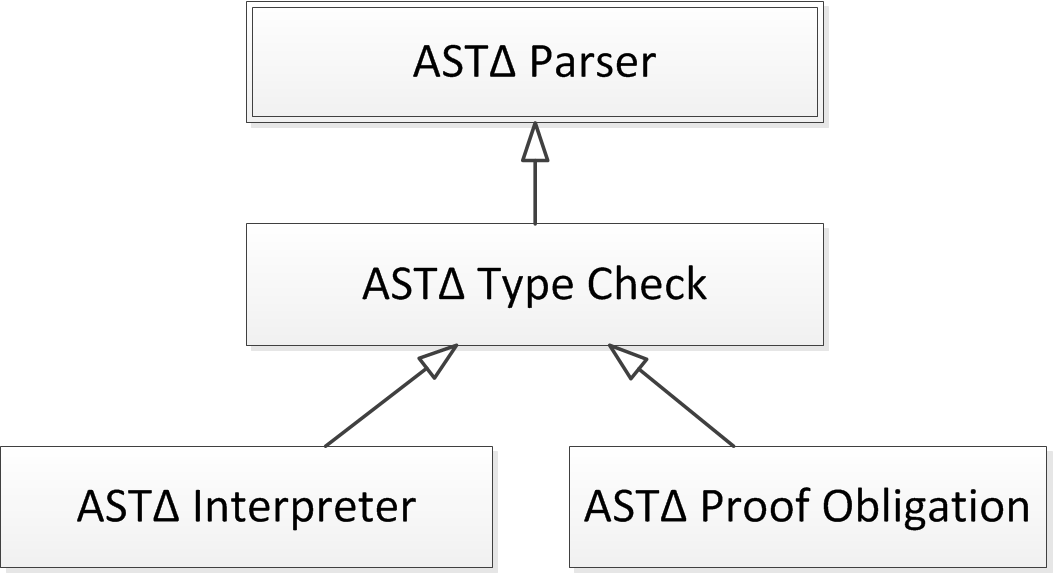
\includegraphics[width=.4\textwidth]{figures/ast_extensions}
\caption{Illustration of AST extensions in Overture.\label{fig:ast_extensions}}
\end{figure}

The extension principle is based on sub-classing from a class-hierarchy where each extended node sub-classes the corresponding node in the base hierarchy. This allows a new extended AST to be used by any implementation that supports its base tree e.g from figure~\ref{fig:ast_extensions} any feature that uses a typed AST can also use an interpreter AST.
To achieve isolation between extensions we require extensions to be declared in a separate file so that a generator (illustrated in figure~\ref{fig:ASTgenExtend}) can combine them into a single tree and generate a converter from the base tree to the extended tree. To illustrate the type check extension listing~\ref{extendedAstEx} shows how expressions are extended with a field for the derived type information.



%Extendibility is important to provide fulfil the goal of an easy extendible platform for new development. But to ensure a stable industrial strength tool such extensions must be isolated, such that new additions do not change the behaviour of existing features. Three kinds of additions has been identified as: adding new nodes, adding new fields to a node or refining a field type of a node. To make it clear what changes are made to the source grammar for a particular feature it was considered a good idea to group new additions in a separate grammar file.
%The initial idea for AST extensions was to create a new derived tree from a source tree where the new tree didn’t have any relation to the source tree. This new tree would be completely independent on the source tree. It would only at generation time copy the structure from the source tree into the target tree. This turned out to be the least efficient way to do development do the lack of reuse because of any utility code made to traverse the tree e.g.collecting names from nodes could not be use one a new extended tree.
%Based on the above a number of requirements for an extended AST has been defined as:
%\begin{itemize}
%\item The extended grammar must only specify additions to a basic grammar.
%\item The extended AST must be generated such that is subclasses the basic AST.
%\item Any visitors and adaptors made for the basic AST must also be able to operate the extended AST excluding the new additions.
%\item A new set of visitors and adaptors must be generated for the extended AST handling both the basic and extended nodes.
%\item A converter which can convert a source AST into its extended version.
%\end{itemize}

%Figure~\ref{fig:ASTgenExtend} illustrates how an extended grammar file can be combined with a source grammar to generate a new extended AST which sub classes the source AST.

\begin{figure}[hpt]
\centering
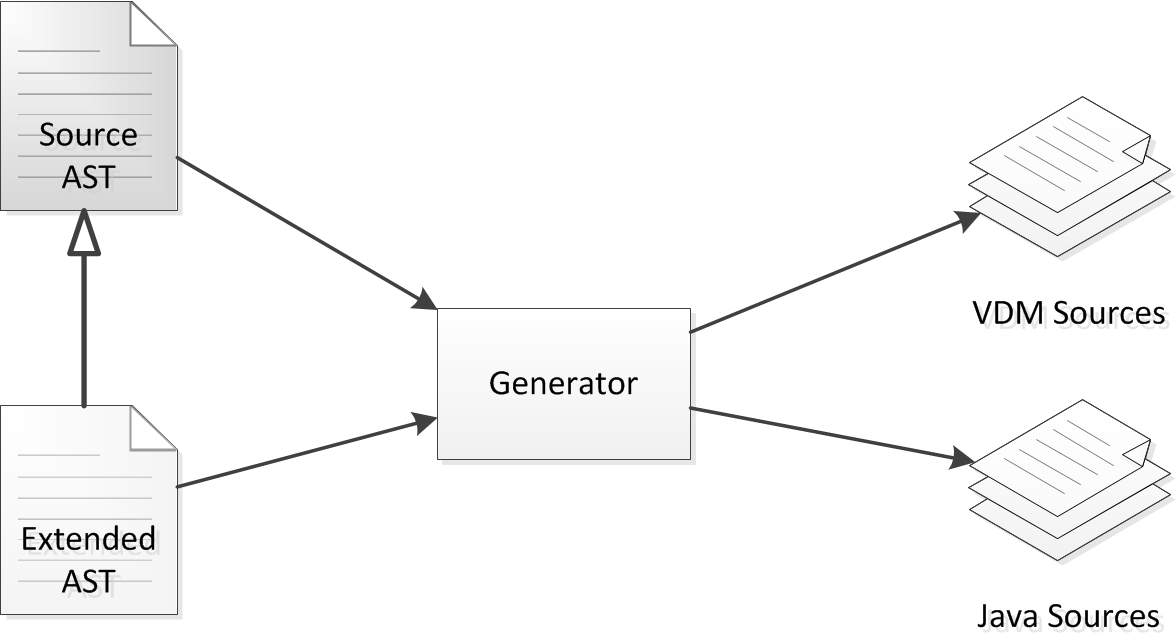
\includegraphics[width=.5\textwidth]{figures/ASTgenerator_extend}
\caption{Extending an existing AST.\label{fig:ASTgenExtend}}
\end{figure}

%The interpreter is one feature which requires a number of additions to the AST. One of such extensions is a new \texttt{breakpoint} expression enabling a user to set a conditional breakpoint during interpretation. A breakpoint expression is not part of the VDM language and should therefore not be added to the source AST but only exist within the interpreter. In listing~\ref{extendedAstEx} the grammar for this extension is shown, the part adding the breakpoint expression to all expressions is left out.

\begin{astlst}[\lstset{caption=Example showing how a type can be added to all expressions.,label=extendedAstEx}]
Aspect Declaration
exp = [type]:type;
\end{astlst}